%%%%%%%%%%%%%%%%%%%%%%%%%%%%%%%%%%%%%%%%%%%%%%%%%%%%%%%%%%%%%%%%%%%%%%%%%%%%%%%%
%2345678901234567890123456789012345678901234567890123456789012345678901234567890
%        1         2         3         4         5         6         7         8

\documentclass[letterpaper, 12 pt, conference]{ieeeconf}  % Comment this line out if you need a4paper

%\documentclass[a4paper, 10pt, conference]{ieeeconf}      % Use this line for a4 paper

\IEEEoverridecommandlockouts                              % This command is only needed if 
                                                          % you want to use the \thanks command

\overrideIEEEmargins                                      % Needed to meet printer requirements.

% See the \addtolength command later in the file to balance the column lengths
% on the last page of the document

% The following packages can be found on http:\\www.ctan.org
%\usepackage{graphics} % for pdf, bitmapped graphics files
%\usepackage{epsfig} % for postscript graphics files
\usepackage{mathptmx} % assumes new font selection scheme installed
\usepackage{times} % assumes new font selection scheme installed
\usepackage{amsmath} % assumes amsmath package installed
\usepackage{amssymb}  % assumes amsmath package installed
\usepackage{enumerate}
\usepackage{cite}
\usepackage{graphicx} % for pdf, bitmapped graphics files
%\usepackage[caption=false]{subfig}
%\usepackage{enumerate}
%\usepackage[english]{babel}
%\usepackage{blindtext}
%\usepackage{booktabs}
%\usepackage{multirow}
%\usepackage{capt-of}
%\usepackage{stfloats}
\usepackage{bm}%bold math
\usepackage{color}
\usepackage{graphicx}
\usepackage{float}
\usepackage{amssymb}
\usepackage{amsmath}
\usepackage{mathtools}
%\title{\LARGE \bf
%Ergodic Coverage Using Sampling-based Motion Planning for Autonomous Exploration In Constrained Environments
%}

\title{\LARGE \bf
Comparison of performance of ORB vs LSD SLAM on Highly-dynamic robots: Snake and Jumping robots
}


\author{Puneet Singhal, Puru Rastogi, and Hadi Salman% <-this % stops a space
%\thanks{*This work was not supported by any organization}% <-this % stops a space
\thanks{$^{1}$Puneet Singhal, Puru Rastogi, and Hadi Salman are with Carnegie Mellon University, Pittsburgh,PA 15213, USA
	{\tt\small (psinghal@,prastogi,hadis@) andrew.cmu.edu}}
}


\begin{document}



\maketitle
\thispagestyle{empty}
\pagestyle{empty}


%%%%%%%%%%%%%%%%%%%%%%%%%%%%%%%%%%%%%%%%%%%%%%%%%%%%%%%%%%%%%%%%%%%%%%%%%%%%%%%%
\begin{abstract}

In this work, we evaluate the performance of ORB and LSD SLAM on highly dynamic robots: Snake Robot and Jumping Robot. Further, we later suggest different ways through which the performance of the evaluated algorithms could be improved on highly dynamic systems.

\end{abstract}


%%%%%%%%%%%%%%%%%%%%%%%%%%%%%%%%%%%%%%%%%%%%%%%%%%%%%%%%%%%%%%%%%%%%%%%%%%%%%%%%
\section{Introduction}
Snake robots are hyper-redundant mobile manipulators which move by slithering over the ground. Whereas GOAT (Gearless Omni-directional Acceleration-vectoring Topology) leg is a jumping monopod robot, that executes jumping gait to move around. Although these 2 robots has completely different topologies, both robot are highly dynamic and hence constitutes a difficult platform to implement localization and mapping algorithms especially visual SLAM. Due to this reason, no attempts were made in this making these 2 robots autonomous and all the motion executed via tele-operation. Furthermore, the planar SEA (Series Elastic Actuator) snake uses pegs/stones to push itself forward. As the camera is mounted on head of the snake robot(as seen in attached Fig.  \ref{fig:snake}), therefore these pegs/stones cause occlusions, which again make the task of mapping and localizing challenging. Another challenge with the snake robot is that the head stays very close to the ground during its motion which causes the horizon to be very high in the image and thus a significant part of the image space is occupied with the ground, which generally has a uniform texture. 

In this work, we evaluate the performance of ORB and LSD SLAM on these highly dynamic and suggest ways to improve their performance in such kind of systems. We start by using benchmark implementation of ORB and LSD on available datasets. This is just to test the successful installation of the implementations on our system. The results for these trials is not presented in the paper. We further evaluate the performance on video collected from a hand-held play station eye camera. Finally, we evaluate their performance on a dataset collected from a camera mounted on the snake robot and GOAT Leg robot. We compare the results from ORB and LSD SLAM with ground-truth values obtained from the Motion-Capture system (OptiTrack).


%%\section{Background}
%%\label{sec:Background}
%%\input{Background}


\section{Implementation and Hardware}
\label{sec:Hardware}
This section describe all the experiments that we have done  using the different algorithms and the different robots setups too.

\subsection{Snake Robot}
The snake robot is a highly articulated robot with a number of joints connected to each other serially, developed at the Biorobotics laboratory at Carnegie Mellon University. An example of this robot is shown in Fig. \ref{fig:snake}. A video of the snake experiments that we did can be reached at https://youtu.be/Cy4igTHlHW4 .
\begin{figure}[t]\label{fig:snake}
	\centering
	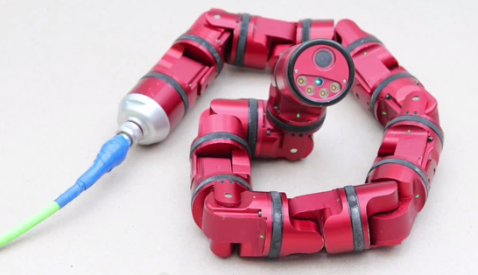
\includegraphics[width=0.7\linewidth]{figures/snake}
	\caption{The snake robot of the Biorobotics Laboratory at CMU, that we used to test and compare how well the ORB and LSD SLAM algorithms work on highly dynamics robots. }
	\label{fig:snake}
\end{figure}


\begin{figure}[t]\label{fig:goat}
	\centering
	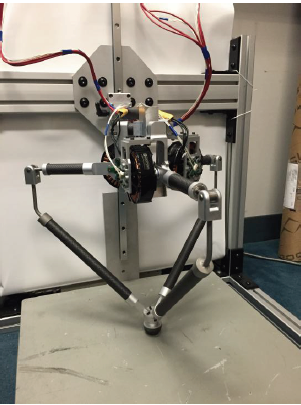
\includegraphics[width=0.7\linewidth]{figures/goat}
	\caption{The Goat Leg (jumping monopod) that we used as one interesting platform to test the SLAM algorithms}
	\label{fig:goat}
\end{figure}

\subsection{GOAT: Jumping Monopod}
The Goat is a jumping monopod developed by the Biorobotics laboratory at Carnegie Mellon University. It has a Gearless Omni-directional Acceleration-vectoring Topology, which is a novel leg design aimed at surpassing all current leg designs in terms of 3D agility. The GOAT leg is modular in that it can be configured with various drive motors and gear-trains for
either DD or QDD. Additionally, the leg can be used in various legged robot morphologies including
monopod, biped, tripod and quadruped. Due to the highly dynamic nature of this robot, we aimed to test and evaluate the state of the art SLAM algorithms on it cause these algorithms migt not behave as well as on mobile robots for example, due to the very fast motion of this robot and the huge shaking of the image while the robot is jumping. A video of the GOAT can be found at https://www.youtube.com/watch?v=n319xVomJTQ.


\section{ORB}
\label{sec:ORB}
ORB-SLAM [1] is a feature-based (ORB features\footnote{ORB are binary features, invariant to rotation and scale (in a certain range), resulting in a very fast recognizer with good invariance to viewpoint})monocular simultaneous localization and mapping (SLAM) algorithm that operates in real time, in small/ large indoor and outdoor environments. ORB are oriented multi-scale FAST corners with a 256-bit descriptor associated. They are extremely fast to compute and match, while they have good invariance to viewpoint. This allows matching them with wide baselines, boosting the accuracy of bundle adjustment, BA. [2] presents the good performance of ORB for place recognition.

\begin{figure}[H]
	\centering
	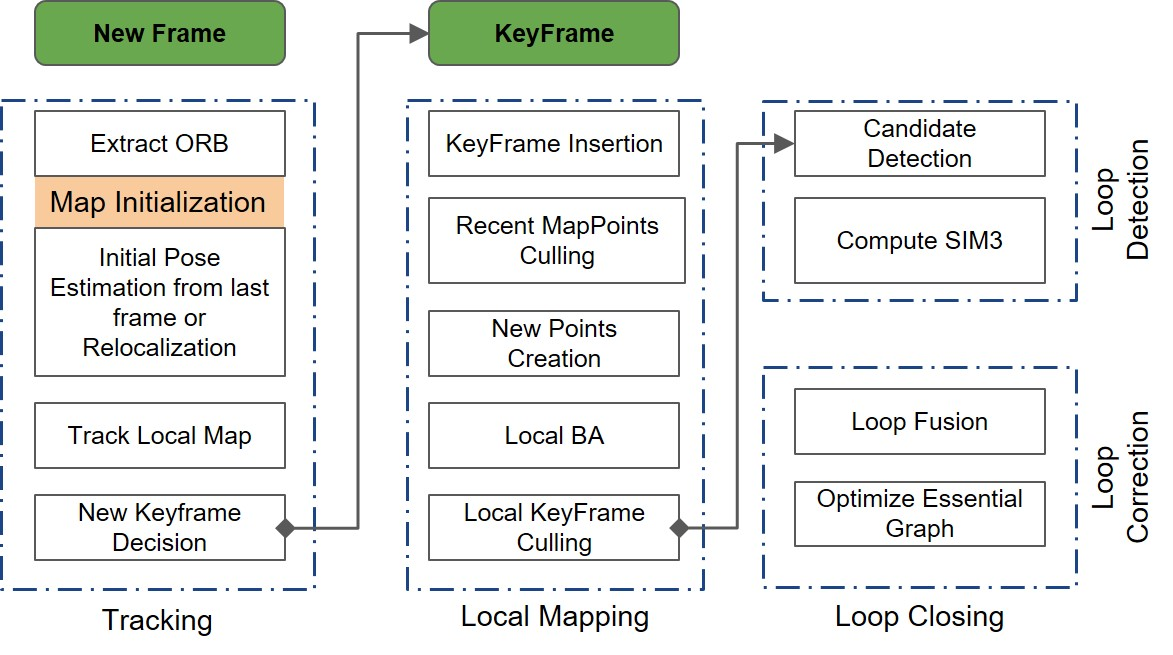
\includegraphics[width=1.0\linewidth]{figures/orb_slam_pipeline}
	\caption{Pipeline of the ORB SLAM algorithm}
	\label{fig:orbslampipeline}
\end{figure}

The main features of ORB-SLAM, are as described below:

a) ORB Features [3]: allow real-time operation without using GPUs. Additionally, it makes it possible to use the same features for all tasks including: tracking, mapping, re-localization, and loop closing.

b) Real-time operation: By using covisibility graph, tracking and mapping are focused in a local covisible area, independent of global map size.

c)Essential Graph: Real-time loop closing based on the optimization of a pose graph.

d)Real-time camera relocalization: Allows recovery from tracking failure and also enhances map reuse.

e)Initialization Procedure: using model selection permits creating initial map of planar and non-planar scenes.

f)Survival of the fittest approach to map point and keyframe selection that is generous in the spawning but very restrictive in the culling. This policy improves tracking robustness and enhances lifelong operation because redundant keyframes are discarded.
\\


The system is comprised of 3 parallel threads, shown in Fig. \ref{fig:orbslampipeline}:

\subsubsection{Tracking} 
A constant velocity motion model is assumed to predict the camera pose and perform guided search of the map points observed in the last frame. Optimization is performed over found correspondences. If tracking is lost, then the frame is converted into bag of words and re-localization is done by finding keyframe candidates from query to the recognition database. Once, estimation of the camera pose is done and an initial set of feature matches, the map can be projected into the frame and more map point correspondences can be searched (Refer to [1] for more details). As there is a mechanism in the local mapping to cull redundant keyframes, the algorithm tries to insert keyframes as fast as possible. This makes the tracking more robust to challenging camera movements, typically rotations. To insert a new keyframe, all the following conditions must be met[1]:

 a) More than 20 frames must have passed from the last global relocalization.


 b) Local mapping is idle, or more than 20 frames have passed from last keyframe insertion.


 c) Current frame tracks at least 50 points.


 d) Current frame tracks less than 90\% points than $K_{ref}$ (reference keyframe $K_{ref} \in K1 $, which shares most map points with current frame)
\\
\subsubsection{Local Mapping} 
with every new keyframe $K_i$, the covisibility graph is updated, adding a new node for $K_i$ and updating the edges resulting from the shared map points with other keyframes. Then the spanning tree is updated linking $K_i$ with the keyframe having most points in common. This is followed by computing the bags of words representation for the keyframe, which will help in the data association for triangulating new points. For a new map point to be retained it must fulfill these two conditions: First, the tracking must find the point in more than the 25\% of frames in which it is predicted to be visible. Second, if more than one keyframe have passed from map point creation, it must be observed from at least three keyframes. Once a map point have passed this test, it can only be removed if at any time it is observed from less than three keyframes. This can happen when keyframes are culled and when local BA discards outlier observations. This policy makes the map contain very few outliers.

\subsubsection{Loop Closing} 
To accept a loop candidate,  three consecutive consistent (keyframes connected in the co-visibility graph) loop candidates should be detected. Similarity transformation is calculated, from the current keyframe $K_i$ to the loop keyframe $K_l$, that represents the error accumulated in the loop. If similarity $S_{il}$ with  enough inliers is found, the loop with $K_l$ is accepted. After this loop fusion is done followed by Essential Graph Optimization.

%[image - ]

\section{LSD}
\label{sec:LSD}
In this section, we briefly describe the LSD algorithm. For more details, the reader is encouraged to refer to the original LSD paper[4].

LSD is a direct featureless monocular SLAM algorithm that allows to build large-scale consistent maps of the environment. The algorithm uses highly accurate pose estimation based on direct image alignment, and reconstructs the 3D environment in real-time as a pose graph of keyframes. The global map is represented as a pose graph consisting of keyframes as vertices with 3D similarity transforms as edges, and this allows for incorporating multi scale environment nature. This algorithm runs in real-time on a CPU.

The algorithm consists of three main parts which are tracking, depth estimation, and map optimization.

For tracking, the rigid posed $\xi \in se(3)$ is estimated with respect to the current keyframe. This part continuously runs at the highest frequency of the pipeline. The depth map estimation part basically uses the tracked frames from part one to either replace the current frame if some conditions are met, or to refine this current frame. The third part which is map optimization consists of including the keyframe that has been replaced in the previous part (depth map estimation), and thus means that it is not going to be refined anymore, into the global map. This parts also contains loop closure and scale drift detection which is done by estimating a similarity transform $\xi \in sim(3)$ using a method called direct-$sim(3)$-image alignment (more details in the original paper[4]).

For initialization, the first keyframe is initialized with random depth map and large variance. LSD best initializes if a sufficient translational camera movement is detected in the first few seconds.

\subsection{Map Representation}
As most state of the art SLAM algorithms, the map is represented as a pose graph of keyframes that captures the dependencies between all the keyframes that are added to the map.

Each keyframe consists basically of an image, an inverse depth map, and variance of the inverse depth map. The edges of the pose graph represents similarity transforms between the keyframes.





\begin{figure}
	\centering
	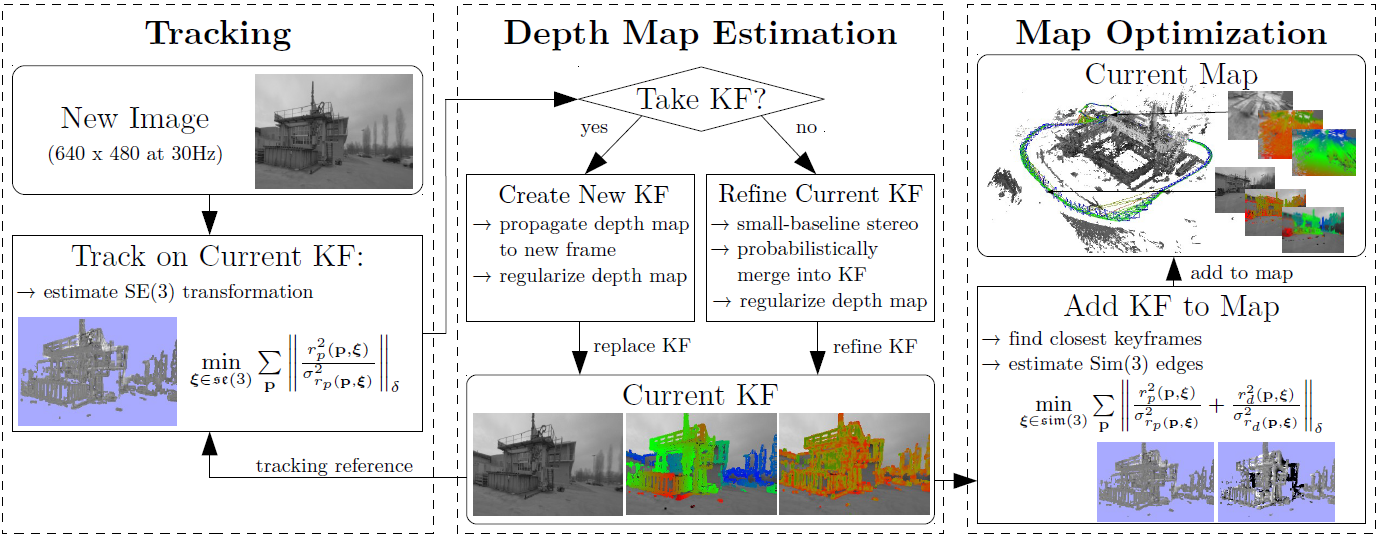
\includegraphics[width=1.0\linewidth]{figures/LSD_summary}
	\caption{Pipeline of the LSD SLAM algorithm [4].}
	\label{fig:lsdsummary}
\end{figure}

\section{Results}
\label{sec:Results}
Evaluation on Dataset packaged with the respective Libraries:
\subsection{Evaluation on Data from Hand-held Camera}
This set of experiment was conducted inside a well lit room while the camera was focussed on a work desk with multiple common objects. Movement of the camera was smooth and had low velocity. Moreover the frame rate of the camera was 60 frames per second.

\subsubsection{LSD}
As could be seen in Fig. \ref{fig:handheldlsd}, LSD performed very well on the video from handheld camera. It was efficiently able to do the 3D reconstruction and tracking. Check the attached video for th results\footnote{Video at https://youtu.be/Btp6bS0udTA}.

\begin{figure}[H]
	\centering
	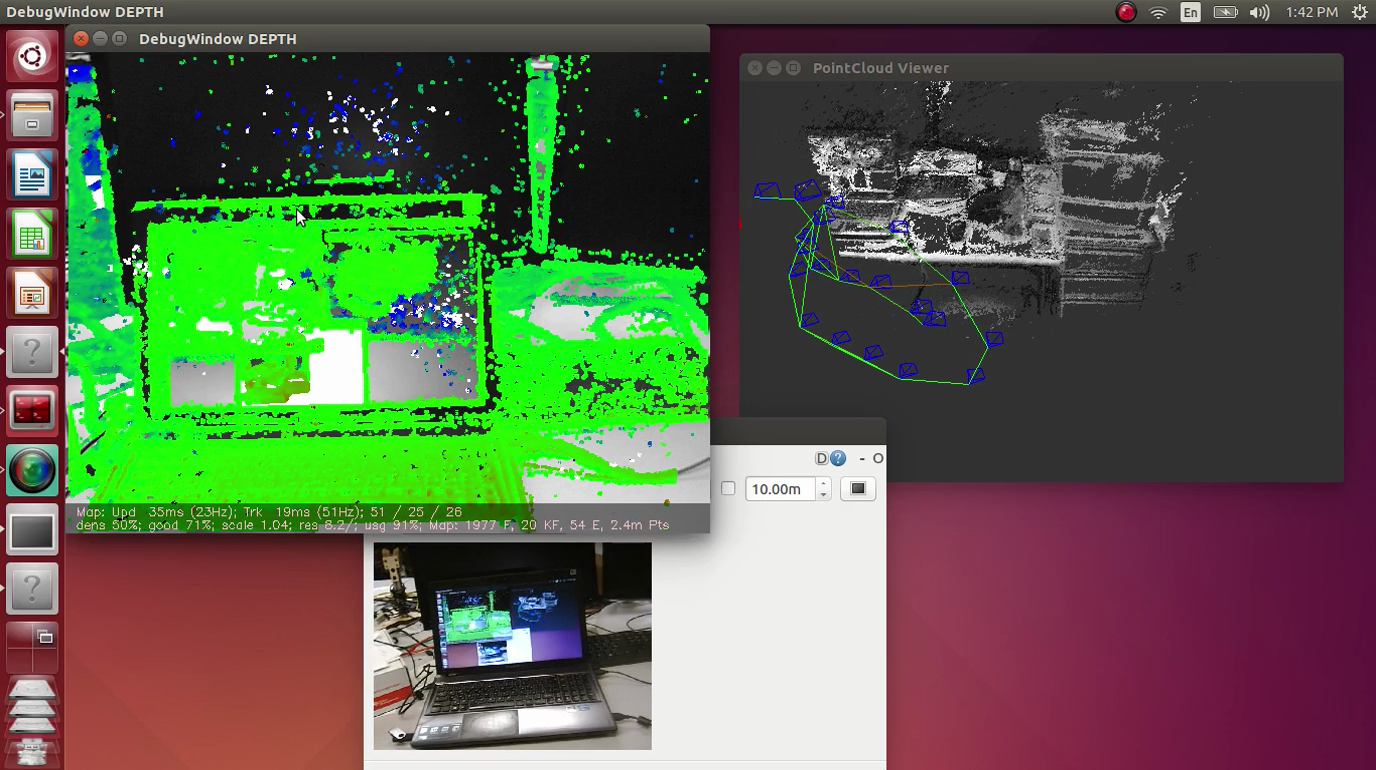
\includegraphics[width=1.0\linewidth]{figures/handHeld_LSD}
	\caption{Snapshot of the off the shelve LSD algorithm implemented using a hand-held camera. The right image shows the keyframes(blue), the trajectory of the camera(green), and the point cloud map at this instance.The left image shows the camera view with the points of the inverse depth map shown in green.}
	\label{fig:handheldlsd}
\end{figure}

\subsubsection{ORB}
For ORB SLAM, initialization is observed using different camera motions. The results are shown in the attached video\footnote{Video at https://youtu.be/1F-ygcA-ZM0\label{xx}}. The initialization time varied with the way camera was moved. If the camera is not moved at all, then it takes around 5.2 seconds to initialize. On the other hand, if we move the camera sideways, the initialization time drops to 3.7 seconds. Interesting thing happened when we do to and fro motion during initialization. To our surprise, the algorithm did not initialize map in this case.

\begin{figure}[H]
	\centering
	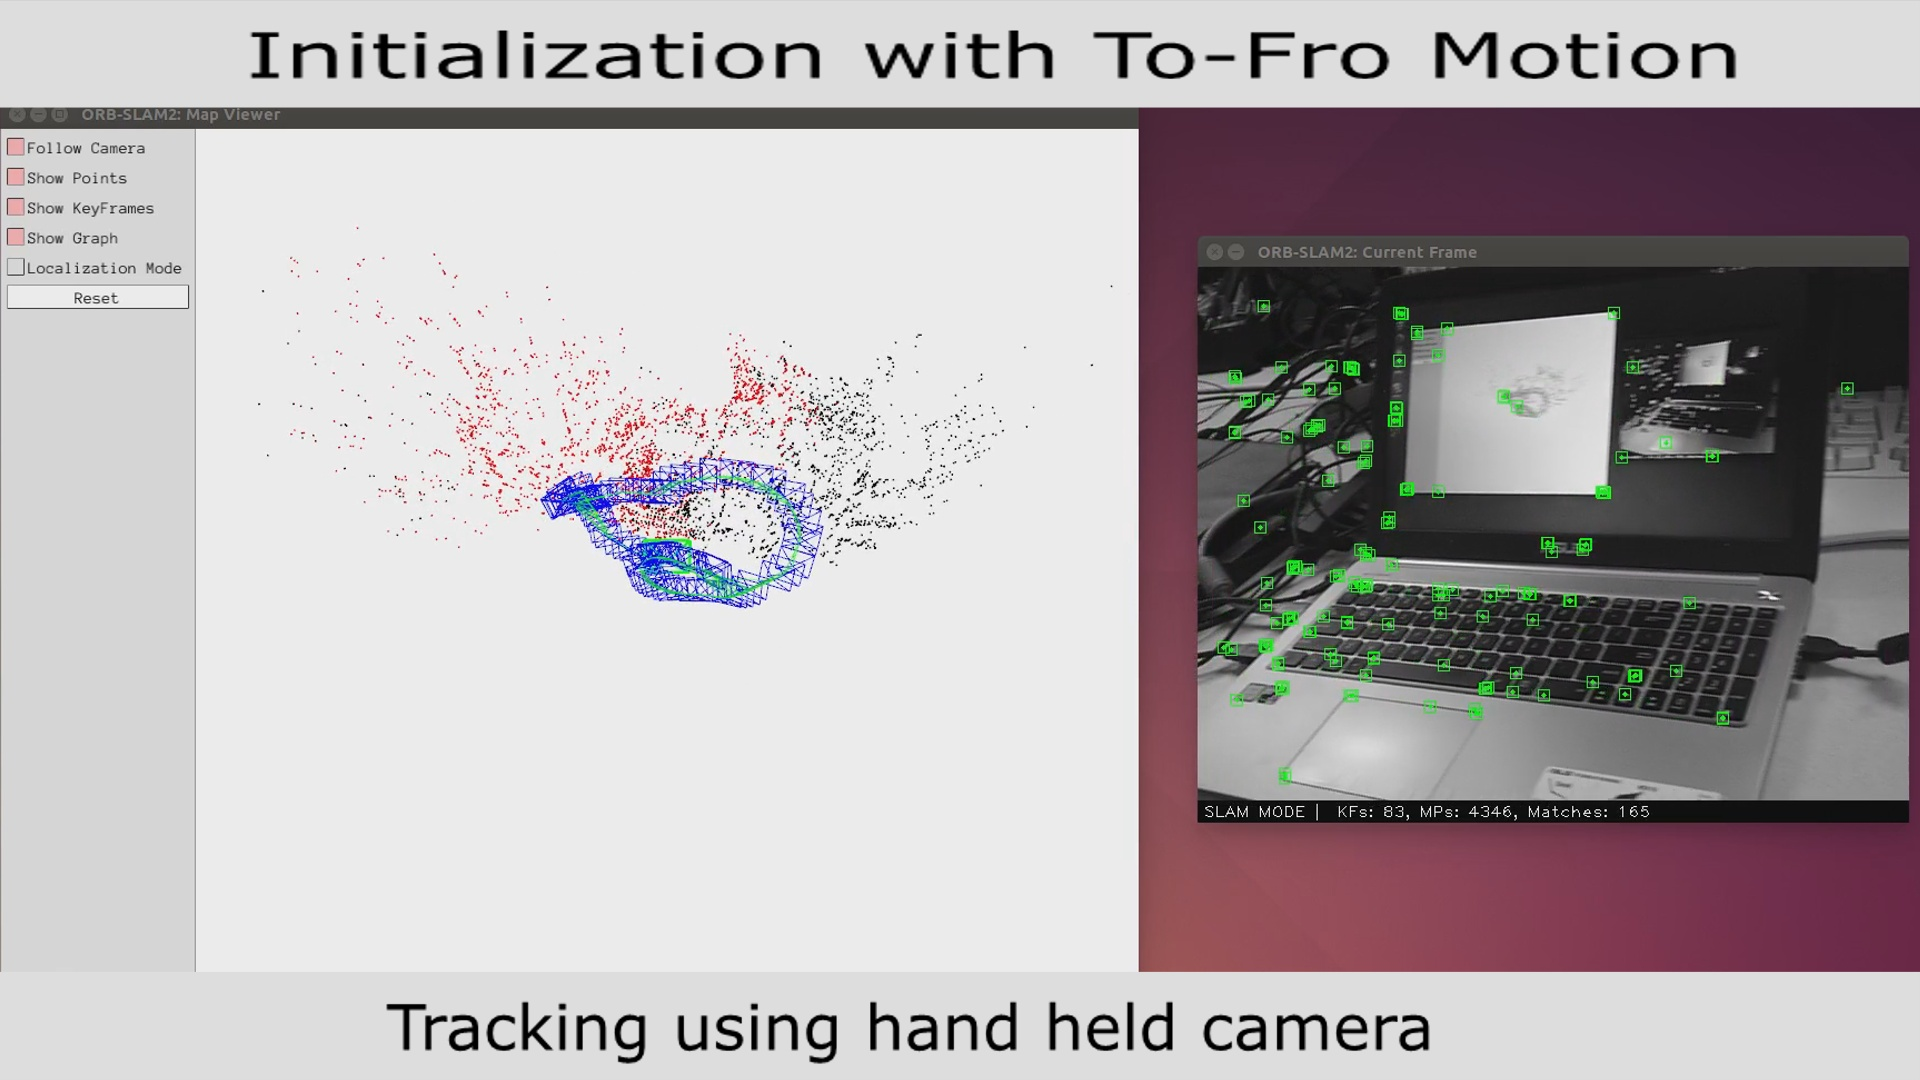
\includegraphics[width=1.0\linewidth]{figures/ORB_handHeld}
	\caption{Snapshot of the off the shelve ORB algorithm implemented using a hand-held camera. The left image shows the keyframes and the point cloud at this instance.The right image shows the camera view with the orb features extracted and shown in green. }
	\label{fig:orbhandheld}
\end{figure}

\subsection{Evaluation on Data from Snake robot}
As mentioned in introduction, the snake moves by pushing the pegs/stones on the ground, and further since the snake’s head moves very close the ground, the video collected from the inbuilt camera in the snake (which is inside its head) majorly contains occlusions by the pegs/stones. In order avoid that and get better video, we mounted a camera over the snake’s head, pointed a little above the horizon. This reduced the issue of high horizon in the image space and occlusion by pegs, although the pegs closer to the camera were still causing occlusion.

\begin{figure}[H]
	\centering
	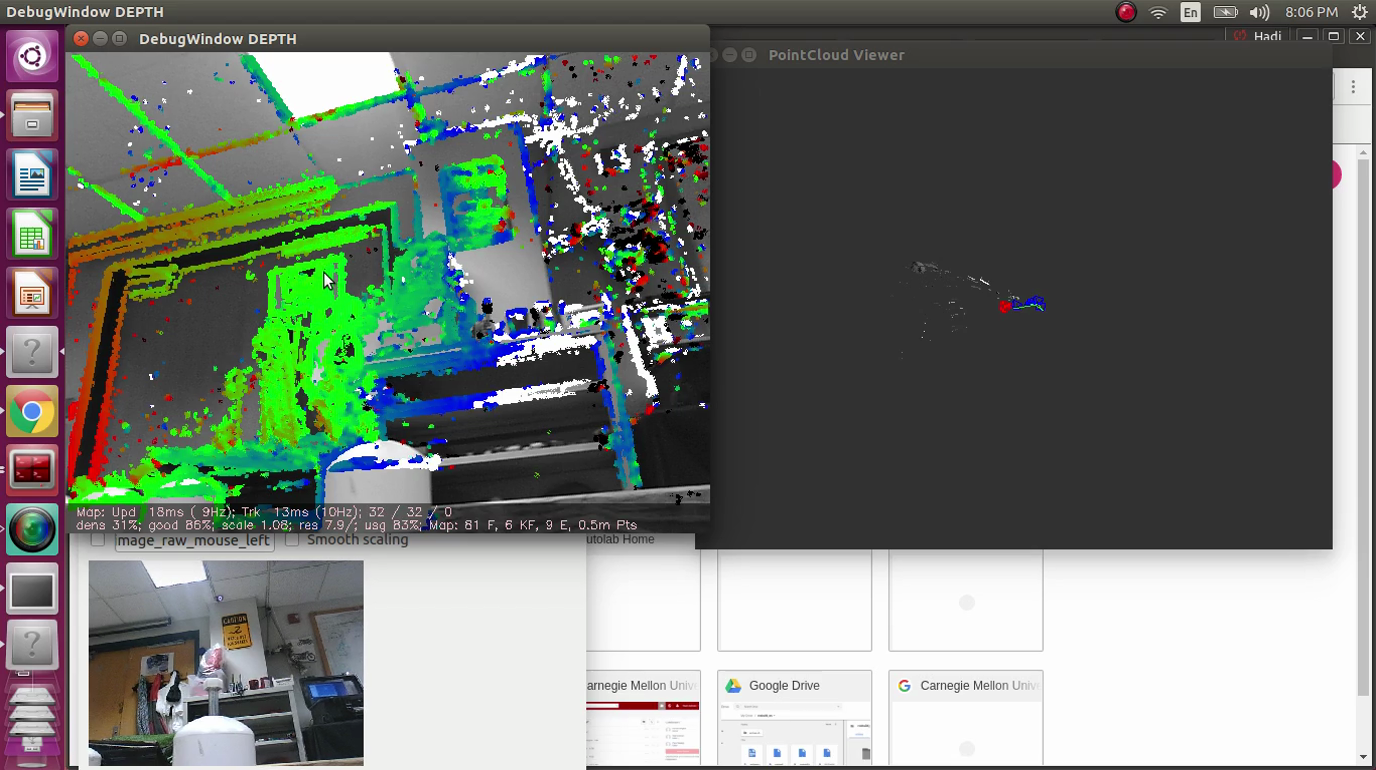
\includegraphics[width=1.0\linewidth]{figures/SNAKE_LSD}
	\caption{Snapshot of the off the shelve LSD algorithm implemented on our Snake robot. The right image shows the keyframes(blue), the trajectory of the camera(green), and the point cloud map at this instance.The left image shows the camera view with the points of the inverse depth map shown in green. As you see in the picture and attached video, the camera looses traking very often due to fast movement of the head of the snake!}
	\label{fig:snakelsd}
\end{figure}
\subsubsection{LSD}
The fast oscillatory and jittery motion of the snake’s head was creating troubles for the LSD. LSD kept loosing the track after every few frames and required initialization as shown in Fig. \ref{fig:snakelsd}. Check the attached video for th results\footnote{Video at https://youtu.be/yBJqJAwULbE}.



\subsubsection{ORB}
It performed better than LSD in terms that it was able to keep track for longer amount of times as shown in Fig. \ref{fig:snakeorb}. During this trial, the truth value of the snake head motion was captured using Opti-track system. The truth value is shown in Fig. \ref{fig:snakerunpscameratrial120170503orb} in blue color. With ORB SLAM, the trajectory derived (scaled by multiplying the coordinates with 10) is as shown in black color in Fig. \ref{fig:snakerunpscameratrial120170503orb}. The difference is quite visible and to our conclusion, the ORB SLAM did not work. We think the reason of failures are: high speed including jerky motions when head gets trapped; some frames with view blocked by pegs resulting in discontinuous tracking; loss of tracking (3 times) during the motion due to poor features. Our proposal going forward is to use high frame rate camera with IMU fusion to recover from loss of tracking and position snake head a little off the ground. Check the attached video for the results\footnote{Video at https://youtu.be/\textunderscore YlEVz5nndY}.

\begin{figure}[H]
	\centering
	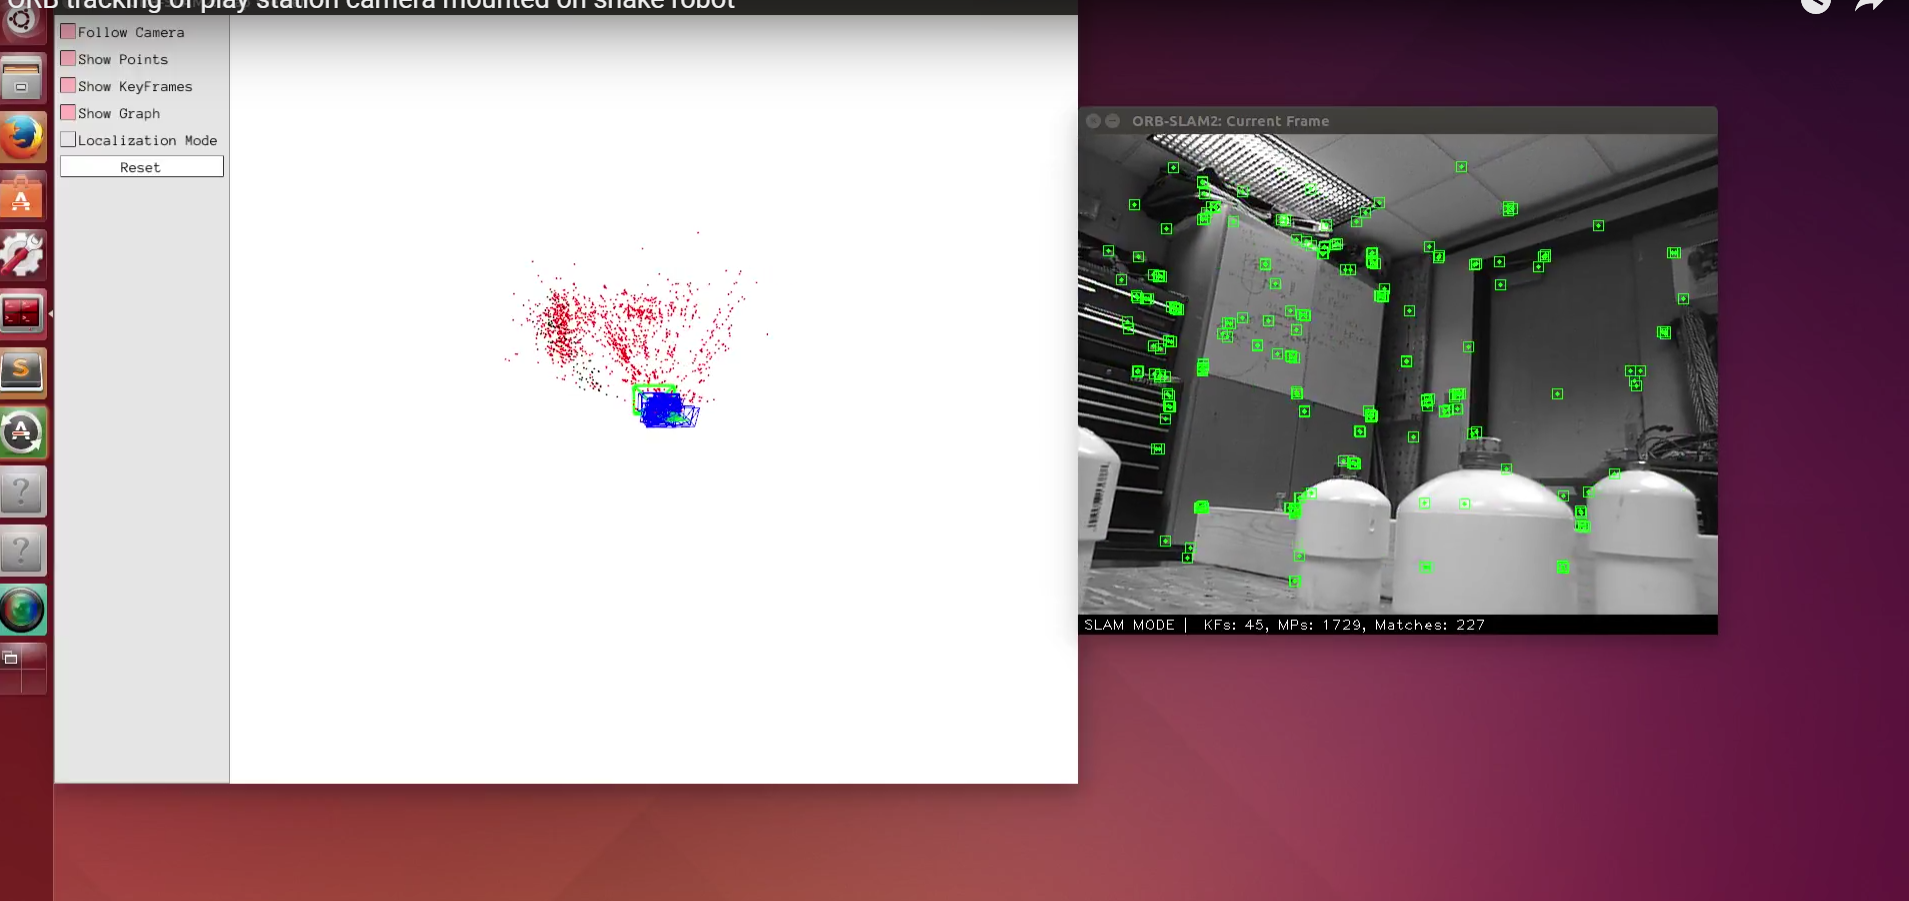
\includegraphics[width=1.0\linewidth]{figures/Snake_ORB}
	\caption{Snapshot of the off the shelve ORB algorithm implemented on our Snake robot. The left image shows the keyframes(blue) and the point cloud map at this instance in red.The right image shows the camera view with the ORB features in green.}
	\label{fig:snakeorb}
\end{figure}

\begin{figure}[H]
	\centering
	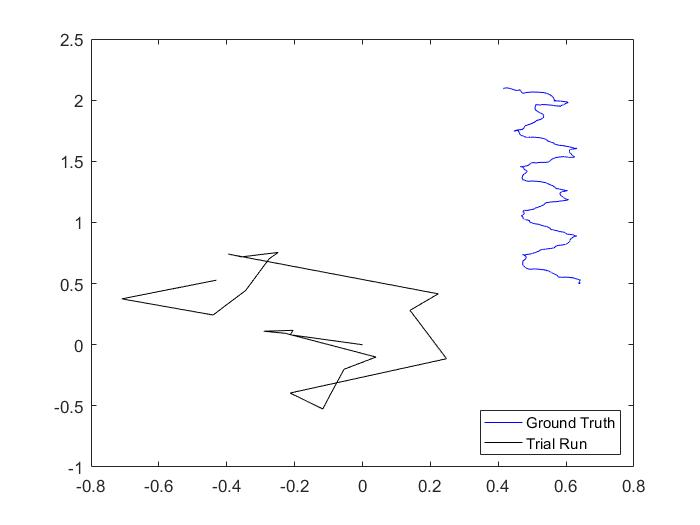
\includegraphics[width=1.0\linewidth]{figures/snakeRun_psCamera_trial1_20170503_ORB}
	\caption{Comparison between the trajectory of the snake robot as obtained by the ORB SLAM algorithm (black) on one hand, and the ground truth captured by a motion capture system (blue) on the other hand.}
	\label{fig:snakerunpscameratrial120170503orb}
\end{figure}

\subsection{Evaluation on Data from Jumping robot}
Unlike the data from the snake mounted camera, the data from jumping robot’s camera does not contain occlusions and high horizon, the only challenge in its data is the jittery or non-smooth motion of the robot.

\subsubsection{LSD}
It worked astonishingly well on the data from jumping robot. It did not loose track, and a snapshot of it could be seen in the Fig. \ref{fig:goatlsd}. Check the attached video for more details \footnote{Video at https://youtu.be/dY85JeTLYEw}
\begin{figure}[H]
	\centering
	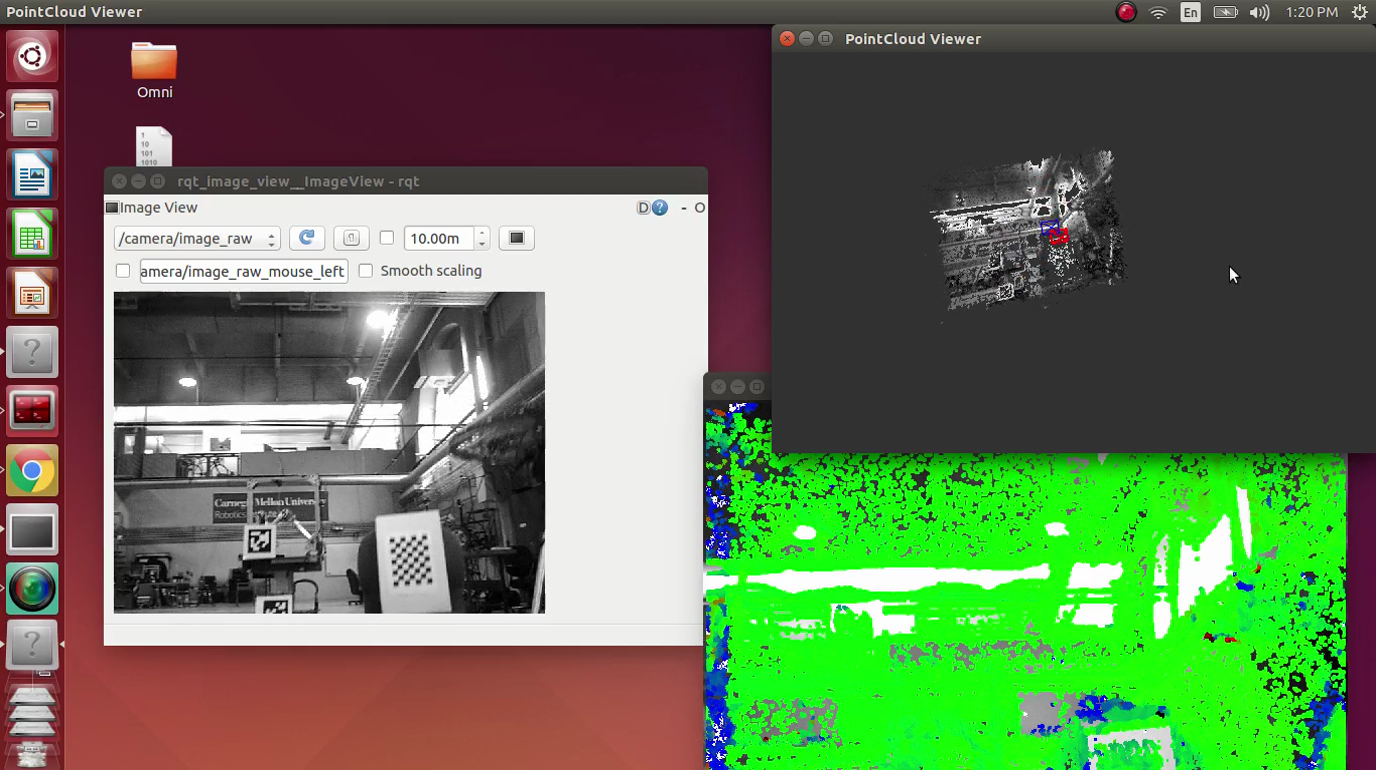
\includegraphics[width=1.0\linewidth]{figures/GOAT_LSD}
	\caption{Snapshot of the off the shelve LSD algorithm implemented on the GOAT robot. The upper right image shows the keyframes(RED) and the point cloud map at this instance in the high bay.The left image shows the camera view, and the lower right image shows the points of the inverse depth map shown in green.}
	\label{fig:goatlsd}
\end{figure}

\subsubsection{ORB}
It was not able to initialize at all on this data. The video was very jittery from the beginning, whereas ORB requires a smoother slow video for initialization



\section{Conclusions}
\label{conclusion}
In this work, we presented the challenges posed by highly dynamic snake robot and GOAT Leg robot, in doing localizing and mapping using monocular vision. We further evaluated two state of the art techniques in SLAM:  ORB and LSD. We started with doing experiments on a hand held play station eye camera where we observed the complications and criticality of initialization process in ORB SLAM. We compared the performance of ORB and LSD SLAM over experiments with planar SEA snake robot and GOAT Leg robot. While for snake robot, LSD did not track at all, it performed really well in case of GOAT leg. This was completely unexpected as GOAT leg moves at high velocity and there are impacts which results in shaky images. ORB SLAM performed completely opposite; the algorithm dit not even initialize in case of GOAT leg but did some tracking in case of snake robot. We shared the shortcomings of both the algorithms for dynamic systems and suggested ways to counter them.

\section{Referneces}

[1] Raúl Mur-Artal, J. M. M. Montiel and Juan D. Tardós., “ORB-SLAM: A Versatile and Accurate Monocular SLAM System,” in IEEE Transactions on Robotics, vol. 31, no. 5, pp. 1147-1163, October 2015.

[2] R. Mur-Artal and J. D. Tard´os, “Fast relocalisation and loop closing in keyframe-based SLAM,” in Proc. IEEE Int. Conf. Robot. Autom., Hong Kong, Jun. 2014, pp. 846–853.

[3] E. Rublee, V. Rabaud, K. Konolige, and G. Bradski, “ORB: An efficient alternative to SIFT or SURF,” in Proc. IEEE Int. Conf. Comput. Vision, Barcelona, Spain, Nov. 2011, pp. 2564–2571.

[4] Engel J., Schöps T., Cremers D. (2014) LSD-SLAM: Large-Scale Direct Monocular SLAM. In: Fleet D., Pajdla T., Schiele B., Tuytelaars T. (eds) Computer Vision – ECCV 2014. ECCV 2014. Lecture Notes in Computer Science, vol 8690. Springer, Cham

\addtolength{\textheight}{-12cm}   % This command serves to balance the column lengths
                                  % on the last page of the document manually. It shortens
                                  % the textheight of the last page by a suitable amount.
                                  % This command does not take effect until the next page
                                  % so it should come on the page before the last. Make
                                  % sure that you do not shorten the textheight too much.

%%%%%%%%%%%%%%%%%%%%%%%%%%%%%%%%%%%%%%%%%%%%%%%%%%%%%%%%%%%%%%%%%%%%%%%%%%%%%%%%



%%%%%%%%%%%%%%%%%%%%%%%%%%%%%%%%%%%%%%%%%%%%%%%%%%%%%%%%%%%%%%%%%%%%%%%%%%%%%%%%



%%%%%%%%%%%%%%%%%%%%%%%%%%%%%%%%%%%%%%%%%%%%%%%%%%%%%%%%%%%%%%%%%%%%%%%%%%%%%%%%
%\section*{APPENDIX}
%Appendixes should appear before the acknowledgment.

%\section*{ACKNOWLEDGMENT}
%The authors would like to acknowledge the assistance of Marin Kobilarov in implementation of the cross entropy method.


%\bibliographystyle{IEEEtran}
%\bibliography{references}
\end{document}


